%APPENDIX D--COMPUTER ASSISTED CURVE FITTING
\newapp
%\section*{Computer Assisted Curve Fitting}
%\addcontentsline{toc}{subsection}{Computer Assisted Curve Fitting}
\label{compassis}

\section*{Introduction}

The preceding appendix showed how many functional relationships
can be reduced to linear relationships by transforming the
variables (e.g., a power law looks like a line if plotted on
log-log paper: $\ln y$ vs.\ $\ln x$) and how to find the parameters
for those functional relationships from the resulting line.
Thus the foundation of ``curve fitting" is determining the
best possible line.  While your eye is an excellent judge of
``best line" we seek an standardized (and automated) method of
determining the ``best line" (and particularly the uncertainty that
should be attached to the resulting slope and intercept parameters).

A solution was published in 1805 by Adrien Marie Legendre in his book 
on determining the orbits of comets. He correctly noted that there is 
arbitrariness in the choice of the best equation, but proposed a solution:

\begin{quote}
Of all the principles that can be proposed for this purpose, I think there 
is none more general, more exact, or easier to apply, than that which we have 
used in this work; it consists of making the sum of the squares of the errors 
[deviation of measurement from equation] a minimum. By this method, a kind of 
equilibrium is established among the errors which, since it prevents the extremes 
from dominating, is appropriate for revealing the state of the system which most 
nearly approaches the truth 
\end{quote}

Thus when we can't make
\begin{equation}
\mbox{``deviation"} =y_i-(A+Bx_i)\label{eq:deviation}
\end{equation}

zero for all the data, we compromise so that some ``deviations" are positive, others negative, 
but the sum of the squares of the ``deviations" for all the data pairs is as small as possible.


\section*{References}

Our treatment of the method of least squares in this appendix is
necessarily brief and incomplete.  At some point in your career, you
are likely to need to learn more
than can be provided here about least-squares fits.  
A good introduction is the book by
Taylor that we have already mentioned several times in this manual:

\begin{itemize}
   \item     John R.  Taylor, {\em An Introduction
to Error Analysis}, second edition, (University Science Books, 1997).
\end{itemize}

The Physics Department requires this book for all second year and
higher laboratory courses, and we recommend it for anyone planning to
major in physics or engineering.  Copies are available in the libraries,
and should also be available or easily ordered at both bookstores.

Two other useful, if more advanced books, are:

\begin{itemize}
\item Philip R.  Bevington \& D. Keith Robinson, {\em Data Reduction and
Error Analysis for the
Physical Sciences} (McGraw-Hill, 2002); and
%
\item  William H. Press et al,
{\em Numerical Recipes: The Art of Scientific Computing}, third edition, (Cambridge
University Press, 2007) especially chapter 15.\\
{\tt http://www.nrbook.com/b/bookfpdf/f15-2.pdf}
\end{itemize}
%In addition, many statistics texts and texts on experimental design and
%data analysis have sections on least-squares fitting.


\section*{Method of Least Squares}

One often wants to find the best equation that describes a set of
experimental data.  The method of least squares 
is the most commonly used technique\footnote{
{\tt http://www.physics.csbsju.edu/stats/fitting\_lines.html}
discusses some other, less common, approaches.
} for  fitting data to a function.  Suppose, for example, that we
have a set of experimental data that lie roughly along a straight
line.  We want to find the ``best" values of slope $B$ and intercept
$A$
for the equation
\[
y = A + Bx
\]
that will describe the data.  The problem is that the
data don't usually fall exactly on any one line.  This is hardly surprising as
the data generally have experimental uncertainties.
For straight-line functions, one can do
reasonably well fitting ``by
eyeball,"---that is, using your best judgment in drawing what appears to
be the best line that describes the data.  But it would be nice
to be able to do a little better.  The method of least squares
provides
a commonly used mathematical criterion for finding the ``best" fit.
Suppose, for example, that our data points are 
$(x_i, y_i)$ for $i=1,2,\ldots N$.

For any point, the deviation
\[
y_i -(A + Bx_i)
\]
is the difference between the
experimental value $y_i$ and the value calculated from the 
(as yet unknown) equation for a
straight line at the corresponding location $x_i$.  Usually this deviation
will have approximately the same magnitude as your experimental
uncertainty or ``error bar." The method of least squares finds the
``best" fit by finding the values of $A$ and $B$ that minimize these
deviations not just for a single data point but for all the
data.  More specifically, it does so by finding the minimum in the
quantity that mathematicians call the reduced chi-squared statistic:


\begin{equation}
\bar{\chi}^{2} \approx {{1} \over {N}} \; \sum_{i=1}^N {{\left[y_{i} -
         f(x_{i})\right]^{2}} \over {\sigma_{i}^{2}}} .
         \label{eq:chisq}
\end{equation}

For our special case in which the function is a straight line, this
equation becomes

\begin{equation}
\bar{\chi}^{2}= {{1} \over {N-2}} \; \sum_{i=1}^N {{\left[y_{i} -
         (A + Bx_{i})\right]^{2}} \over {\sigma_{i}^{2}}}
         \label{eq:chisq_line}
\end{equation}

where $N$ is the number of data points, $f(x)$ is the fitting
function,
and the $\sigma$'s are the standard deviations introduced in Appendix
A---more intuitively, the uncertainties (or ``errors") associated
with
each $y$ value.  In the second expression, $N-2$ is the 
number of ``degrees of freedom" for $N$ data points fit to a line.

Once a fit has been found (i.e., we have found  the values of $A$ and $B$
that minimize reduced chi-square), we need some way of determining
how good the fit is, that is: are the data well described by this line
or is the relationship more complex (for example, quadratic).
%  If, for example, we inadvertently attempt
%to fit data that lie along some curve to a straight line
%fitting function, our fitting program will give an answer, even though
%the fit is a poor one in the sense that the fitting function
%will not go through many of the error bars.
One good visual check is to compare the fitted
solution to the data graphically --- that is, plot the function and
your data on the same graph, and see how well the function
describes your data.  Another easy way to check the fit is to see
if the deviations %--- that is, the difference between the data
%points $y_{i}$ and the calculated values $A + Bx_{i}$ --- 
are significantly
larger than the corresponding uncertainty or show a pattern, for example, being
consistently positive in some ranges of $x$ and negative in others.  These deviations are listed on the 
computer-generated fit report.
%and will be easy to inspect.

{\bf IMPORTANT:}  \label{par:chi_square} It turns out that our reduced chi-squared statistic
provides another, more abstract criterion for goodness of fit.
Statistical theory tells us that a good fit corresponds to a reduced
chi-squared value of about one.  
%A proof is beyond the scope of
%this manual; see Taylor or any good statistics text for a more
%complete discussion.

It is not hard to understand this result intuitively.
Notice that each term in the chi-square sum, (deviation/error)${}^2$,
should be nearly one and we have $N$ such terms, which in the end
are divided by $N-2$.
% Note that the quantity we are minimizing, the reduced
%chi-squared, depends on the size of the experimental
%uncertainties (that is, the $\sigma$'s in Eq.~\ref{eq:chisq} above)
%as well as the
%deviations.   Thus, the reduced chi-squared value will be about one
%when the deviations --- the differences between the $y$ values
%and the fitting function, represented in Eq.~(\ref{eq:chisq}) by the
%quantities $ \left[y_{i} -  (A + Bx_{i})\right] $ --- are about
%equal to the size of the $y$ error bars, the $\sigma_i$.
That is reduced chi-square represents something like the average
deviation divided by the expected deviation squared.  
Take a look at the reduced chi-square equation, and be sure you understand
this point.  
%Larger values of the $\sigma$'s in this equation will
%lead to a smaller reduced chi-squared statistic, and vice versa.

More or less arbitrarily, the fitting
program assumes that any value of reduced chi-square
($\bar{\chi}^2$) between 0.25 and 4 represents a
reasonably good fit.  Otherwise, the program warns you that your fit
may not be valid.

There are two reasons why the value of the reduced
chi-squared statistic might not be close to one.  First, you may have
picked an inappropriate fitting function: If your data describe a
curve and you try to fit them to a straight line, for example, you
will certainly get a bad fit!  Look at a graph of your data along with
the fitting function and see how well the two agree.

Second, you may have overestimated or underestimated your experimental
uncertainties.  In this case, your fit may be all right, but your
uncertainties are nevertheless leading to a value of reduced
chi-squared significantly larger or smaller than one.  In this case,
{\bf DO NOT} try to correct the problem by guessing at the errors until you
get a reasonable reduced chi-squared value!!  Instead, see if you can
figure out why your estimates of the experimental error are off.  If
you can't, talk to your instructor or simply say in your lab notebook
that your estimates of experimental error are apparently wrong, and
you are not sure why.  This approach is not only honest, it is much
more in the spirit of scientific inquiry!  And as a practical matter,
whoever grades your lab is more likely to be favorably impressed by a statement
that you don't understand something than by an obvious attempt to
``fudge" your error estimates!



\subsection*{Using Errors in Both $x$ and $y$}

Most treatments of the method of least squares, and many computer
programs that use it, assume that the only experimental uncertainties
are in $y$ --- in other words, that any uncertainty in $x$ can be
neglected.  This assumption is reasonably accurate in a surprising
number of cases.  Nevertheless, in many experiments there will be
significant uncertainties in both the $x$ and $y$ values and our fitting
program is designed to include both of them.  

\subsection*{An Example, with Details}
\begin{figure}
\begin{center}
\subfigure[Constant curves (ellipses) for $\bar{\chi}^{2}$ are displayed 
as a function of the test line's slope $B$ and $y$ intercept $A$.
The minimum value of $\bar{\chi}^{2}$
%(14041/8064$\approx$1.74) 
occurs at the point $R$.  The constant curves
are for $\bar{\chi}^{2}$ ${1\over 6}, {2\over 6}$, and ${3\over6}$
above that minimum.  
%Points $Q$ and $R$ are the extreme vertical and right points  on
%the constant curve $\bar{\chi}^{2}=\mbox{minimum}+{1\over 6}$.
  \label{fig:contour.exC2}]{\parbox[b]{2.6in}{\begin{center}
{\resizebox{2.55in}{!}{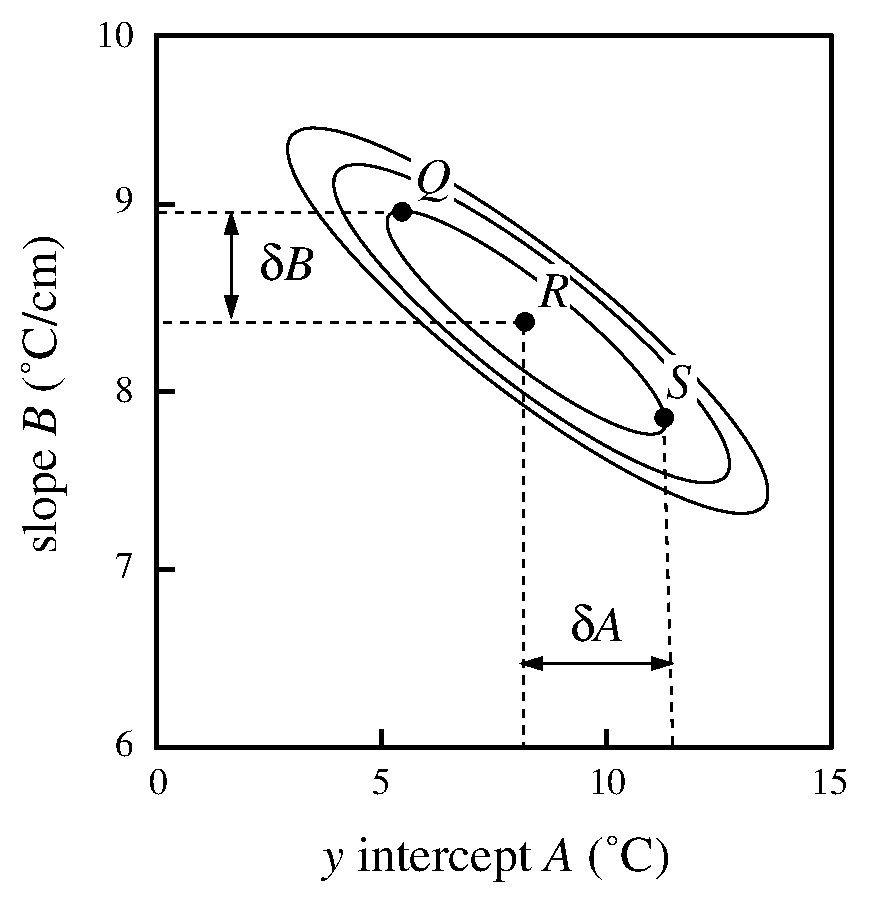
\includegraphics{exampleCs.eps}}} 
\end{center}
}}$\quad$
\subfigure[The dashed lines show the extreme cases corresponding to points $Q$ 
(maximizing the slope) and $S$ (maximizing the $y$ intercept).
The best curve, corresponding to the $\bar{\chi}^{2}$ minimum $R$, is displayed as a solid
line.
 \label{fig:plot.exC2}]{\parbox[b]{2.6in}{\begin{center}
\rotatebox{-90}{\resizebox{2.8in}{!}{\includegraphics{exampleC2_plot.eps}}} 
\end{center}}}
\end{center}
 \caption{Minimizing  $\bar{\chi}^{2}$ for the dataset in Table~\ref{table:tempD}. \label{fig:d1}}
\end{figure}
Consider again the data presented on page \pageref{table:temp}
(where this time we ignore the error in $x$):

\begin{table}[h]
\begin{center}
\begin{tabular}{|cl|}
\hline
$d$ (cm) &\hspace{5pt} $T$ ($^{\circ}$C)  \\ \hline
1& \hspace{5pt} 16 $\pm$ 4  \\
2& \hspace{5pt} 18  \\
3& \hspace{5pt} 35  \\
4& \hspace{5pt} 44  \\
5& \hspace{5pt} 58  \\
6& \hspace{5pt} 62  \\
7& \hspace{5pt} 64  \\
8& \hspace{5pt} 70  \\  \hline
\end{tabular}
\end{center}
\caption{Sample data of temperature as a function of distance along a metal
         rod.  \label{table:tempD}}
\end{table}

If we plug this data into our definition of reduced chi-square $\bar{\chi}^{2}$ (Eq.~\ref{eq:chisq_line})
we find:
\begin{equation}
\bar{\chi}^{2}= { 19945 - 734 A + 8 A^2  - 4006 B + 72 AB + 204 B^2 \over 96}
\end{equation}
(Each term in the sum is a quadratic form in $A$ and $B$; sum those 8 quadratic forms
and divide by $N-2=6$ yields the above.  It is a mess to confirm this by hand; I used
{\em Mathematica}.) So reduced chi-square $\bar{\chi}^{2}$ is a simple quadratic
function of $A$ and $B$. We can find the minimum of this function by finding the
point where the derivatives are zero:
\begin{eqnarray}
{\partial\bar{\chi}^{2}\over \partial A}&=& { -734 +16 A +72 B  \over 96} =0 \\
{\partial\bar{\chi}^{2}\over \partial B}&=& { -4006 + 72 A + 408 B  \over 96} =0 \\
\end{eqnarray}
The result is $(A,B)=(115/14,703/84)\approx(8.21, 8.37)$.

Reduced chi-square $\bar{\chi}^{2}$ is a function of two variables much as
the height of a mountain range is a function of the $x,y$ location on the surface of the Earth.
We can display such height information in the form of a topographical map, where we
connect with a line all the points that are at the same altitude.  In a similar way
we can display the function $\bar{\chi}^{2}(A,B)$, by showing the collection of
points where $\bar{\chi}^{2}(A,B)$ equals some constant.  (See Figure~\ref{fig:contour.exC2}.)
Since $\bar{\chi}^{2}(A,B)$
is a simple quadratic form the resulting constant curves are ellipses,
and the `topography' is quite simple with a single valley, oriented
diagonally, with minimum at the point $R$.  The uncertainly in the best fit
parameters is determined by topography around that minimum: how much
can a parameter vary before the resulting line is a detectably worst fit.
The definition of `detectably worst' is where the chi-square sum has increased
by one unit above the minimum.  The extreme points $Q$ and $S$ are
displayed in the above figure along with the corresponding lines.

In more complicated situations, the chi-square topography can become much more
complex, with several local valleys (which makes finding the global
minimum more difficult).  In the simplest cases (like
that discussed above) the derivatives of chi-square are easily solved linear 
equations with a unique solution (hence just one valley).  These cases are
known as linear least squares.

\label{par:small.error}You may be surprised at the relatively small range of variation implied by the
parameter errors and displayed in Fig.~\ref{fig:plot.exC2}.  Recall that the
parameters are estimates of average behavior revealed by the assumed
unbiased deviations.  So much as the standard deviation of the mean
(discussed on page \pageref{sdev.mean}) is smaller than the
standard deviation (and in fact can get arbitrarily small with sufficiently
large data sets), so too the parameter uncertainties become increasingly
small with large data sets.  As a result the systematic errors must dominate
the random errors for sufficiently large data sets, in which case the computer reported
errors are not relevant. 

\section*{Introduction to \WAPP}

There are many computer programs that can do least-squares fits.  In
this laboratory we will use the web-based program \WAPP located at:\\
\verb+http://www.physics.csbsju.edu/stats/WAPP2.html+.\\ I suggest you add
it to your favorites\footnote{a Google for ``wapp+" will provide a link or
you can hit the statistics link on the Physics homepage: {\tt www.physics.csbsju.edu}}.

On the opening page of \WAPP you must report the format of your
data, particularly for the uncertainty in your data:

\begin{itemize}
\item No $y$ error

Select this if your $y$ data has no error (unlikely) or if you
have no estimate for that error (rare) or if you have been told that
the error is ``negligible".

\item Enter a formula for $y$ error

It is not uncommon to have a simple formula for your errors.  In the simplest possible
case your error may be a constant.  Often you will know the error as a fraction (or percentage)
of the $y$ value.  Very occasionally you may know a fairly complex formula for the error. (For example,
in Physics 200, one error is calculated from: {\verb|(y^2+1)*pi/90|}.)  If you have such
a formula, you may supply it to the program to calculate the errors for you.
Alternatively you could use a spreadsheet or calculator to calculate those errors
and just enter them along  with your data.

\item Enter $y$ error for each data point

Sometimes errors are estimated as part of the experiment by repeating the experiment
and looking for deviations.  In this case the errors are likely to be different for
each data point and there will be no formula to apply.
\end{itemize}

Exactly analogous boxes must be checked to indicate the nature of $x$ errors.

There are two ways of entering your data into the computer: copy \& paste from
a spreadsheet (the usual approach because using a spreadsheet is often required
for other  parts of the experiment) or entering each number into its own box on the web page.
I would always opt for the former (``bulk" or copy \& paste), but if you really want
to you may use the latter (``pointwise data entry").

On the second page of \WAPP you must enter your data and select 
which function applies to your data.  Usually you will paste your data
into the web-form from a spreadsheet.  Obviously you must tell \WAPP
which column contains which data.  Sometimes you will have a column of irrelevant 
data between the $x$ and $y$ data: no problem, just tell \WAPP
to Ignore the irrelevant column.

{\bf Note: } The apparent cells and columns in the ``Block Copy \& Paste" web-form,
in fact, have no meaning: its just an image to remind you that this area will be
filled by pasting data from a spreadsheet.  The pasted data does not have to line up
in columns (the white space between the numbers is what denotes column boundaries).
You do need to assure  that the number of numbers in each row matches the number
of columns not selected as None.  In addition, pasted data must be numbers not text
(for example: column labels). Finally an extra Return at the end of the last
data item may avoid IE transfer problems.

When you Submit Data, the third page of \WAPP arrives: this is your
``fit report".  Almost always you will want to select the top region of this page,
print it out, and tape it into your notebook.  Here is page generated by the
data from Table~\ref{table:tempD}.

An analysis of data submitted by computer: linphys1.physics.csbsju.edu on 1-APR-2008 at 
13:35 indicates that a function of the form:\\
---{\bf Linear}--- $y=A+Bx$\\
can fit the 8 data points with a reduced chi-squared of 1.7\begin{verbatim}
                FIT
 PARAMETER     VALUE        ERROR
   A =          8.214        3.1    
   B =          8.369       0.62    
 
 NO x-errors

                   ACTUAL     ERROR IN         CALCULATED   DEVIATION
 POINT    X          Y            Y                Y        FROM FIT
   1     1.00       16.0     +-  4.0              16.6      -0.583    
   2     2.00       18.0     +-  4.0              25.0       -6.95    
   3     3.00       35.0     +-  4.0              33.3        1.68    
   4     4.00       44.0     +-  4.0              41.7        2.31    
   5     5.00       58.0     +-  4.0              50.1        7.94    
   6     6.00       62.0     +-  4.0              58.4        3.57    
   7     7.00       64.0     +-  4.0              66.8       -2.80    
   8     8.00       70.0     +-  4.0              75.2       -5.17    \end{verbatim}
{\small \bf Data Reference: 626A}

It is perhaps worth reminding you that computers are usually ignorant of sigfigs
and units:
I would report these results as: $A=8\pm3\;{}^{\circ}{\rm C}$ and
$B=8.4\pm.6\;{}^{\circ}{\rm C/cm}$. Alternatively $A=8.2\pm3.1\;{}^{\circ}{\rm C}$ and
$B=8.37\pm.62\;{}^{\circ}{\rm C/cm}$ is also OK; other possibilities are incorrect
and will result in lost points.

The {\small \bf Data Reference: 626A} at the bottom is useful and should be retained.  
If some problem (e.g., a computer crash) should occur, it is likely that this reference
will allow you to get a copy of your data from the web.

The bottom part of this page allows you to make various types of plots of your results.
If you click on ``Make Plot" a fourth page pops up with links to the actual plots.
Most commonly you will click on the PDF File, Adobe Acrobat will launch and your plot
will be displayed, and if desired printed.


\paragraph*{How to enter formulas:}
The usual syntax applies: + $-$ * / for add, subtract,
multiply, and divide respectively; \verb+^+ or ** for powers.  
Please note:
\begin{eqnarray}
{\tt A/B*C} &=& {AC\over B}\\
{\tt A/(B*C)} &=& {A\over BC}
\end{eqnarray}

\paragraph*{Mathematical functions for formulas:}
\begin{tabbing}
ABS \hspace*{1in} \=  ACOS \hspace*{1in}  \= ASIN \hspace*{1in} \=  ATAN \\
COS    \>  COSH  \>  ERF  \>  ERFC \\
EXP     \>  INT   \>  LOG   \>  LOG10   \\
NINT     \>  RAN   \>  SCALE     \>  SIGN  \\
SIN    \>  SINH   \>  SQRT    \>  TAN  \\
TANH       \>  GAMMA \>  K   \>  NORM \\
INORM     \>  PI \\
\end{tabbing}

